%%%%%%%%%%%%%%%%%%%%%%%%%%%%%%%%%%%%%%%%%%%%%%%%%%%%%%%%%%%%%%%%%%%%%%%%
\chapter{Applicazioni della CP alla complessità aritmetica}
\label{chp:matmul}
%%%%%%%%%%%%%%%%%%%%%%%%%%%%%%%%%%%%%%%%%%%%%%%%%%%%%%%%%%%%%%%%%%%%%%%%


Conoscere il rango CP di tensori che rappresentano applicazioni multilineari può rivelare
informazioni sulla complessità asintotica e fornire algoritmi con complessità ottimale per la loro
valutazione. Proviamo a formulare il problema.\todo{sistemare}

\todo{Controlla che non ci sia ambiguità nel riferirti a mappe/forme bilineari: $ \psi : U\times V
\to W $ è una forma bilineare se $ W = \K $, altrimenti chiamala mappa bilineare}
\todo{rinomina le forme bilineari con $ \varphi $ invece che $ f $}

\missingfigure{Breve introduzione per questo capitolo}

\section{Mappe multilineari e moltiplicazione tra matrici}
\label{sec:tensor_bil}

\todo{Fix conflicting notation!}

Siano $ M,N,P $ spazi vettoriali di dimensione finita, di dimensione $ m,n,p $ rispettivamente. Una forma bilineare è una mappa $ f : M \times N \to
P$ lineare in ogni componente, in altre parole tale che $ f(m, \cdot) $ e $ f(\cdot,n) $ sono
lineari per ogni $ m\in M $ e $ n\in N $. In maniera analoga si definiscono le mappe trilineari $ f:
M_1 \times M_2 \times  M_3 \to P$.

\begin{definition}[Moltiplicazione matriciale]
 Fissati degli interi positivi $ m,n,p $, la moltiplicazione tra due matrici $  m\times n $ e $ n \times p $ è una mappa bilineare
 \begin{equation*}
   \begin{aligned}
     \algob{m,n,p} \colon \C^{m\times n} \times \C^{n\times p} &\to \C^{m \times p} \\
     (A,B) &\mapsto C = AB.
   \end{aligned}
 \end{equation*}
 Spesso ci riferiremo a $ \algob{m,n,p} $ chiamandolo ``algoritmo'', ad esempio nel contesto degli algoritmi di
 moltiplicazione veloce.
\end{definition}

\begin{remark}
  La bilinearità della mappa sopra segue immediatamente dalla definizione
  \begin{equation}
    \label{eq:matmul_component}
    (AB)_{ij} = \sum_{k=1}^N a_{ik}b_{kj},
  \end{equation} dove $ i = 1, \ldots, M $ e $ j = 1, \ldots,P $.
\end{remark}

\begin{remark}
  \label{rmk:triliear_matmul}
Possiamo vedere la moltiplicazione tra matrici anche come una mappa trilineare
  \begin{equation*}
    \begin{aligned}
      \C^{M\times N} \times \C^{N\times P} \times \C^{M\times P} &\to \C \\
      (A,B,C) &\mapsto \mathop{trace}(ABC)
    \end{aligned}
  \end{equation*}
\end{remark}
\todo{giustifica se necessario}


\todo{se riesci muovi al capitolo 1}
\subsection*{Rappresentazione in coordinate di una forma bilineare}

Sfruttando l'isomorfismo con lo spazio vettoriale standard, possiamo
rappresentare una forma bilineare $ f \colon X \times Y \to Z $ come un tensore nel seguente modo: fissato $ k \in \{1, \ldots, p\} $ e
considerata $ f_k : X \times Y \to \R $, esiste una matrice $ M \in \R^{m \times n} $ tale che $
f_k(x,y) = x^{\top}My$ per ogni $ (x,y) \in \R^m \times \R^n $. Scrivendo ogni componente di $
f = \begin{bmatrix} f_1 \\ \vdots \\ f_p \end{bmatrix}$ in questa forma, otteniamo un tensore $ T \in \R^{m \times n\times p} $ tale che le sue slice
frontali rappresentino ognuna delle $ p $ forme bilineari $ f_k $, ossia che
\begin{equation}
  \label{eq:b_k_bil}
  f_k(x,y) = x^{\top}T_{:,:,k}y = \sum_{i=1}^m\sum_{j=1}^n T_{i,j,k}x_iy_j, \text{ per ogni
  } k = 1, \ldots, p
.\end{equation}
In forma tensoriale,
\begin{equation}
  \label{eq:b_tuv}
 f(x,y) = \begin{bmatrix} f_1(x,y) \\ \vdots \\ f_p(x,y) \end{bmatrix} = \begin{bmatrix}
 x^{\top}T_{:,:,1}y \\
\vdots \\ x^{\top}T_{:,:,p}y \end{bmatrix} = T \ttm[1] x^{\top}
 \ttm[2] y^{\top}.
\end{equation}
\begin{remark}
  Questa procedura si estende (passando alle coordinate) anche al caso in cui le entrate di $ x $ e $ y $ siano oggetti
  algebrici più complessi di scalari, ad esempio vettori o matrici.
\end{remark}



\section{L'esponente della moltiplicazione tra matrici}

In questo capitolo useremo il seguente modello computazionale per il calcolo della complessità, per
calcolare costi computazionali anche su campi infiniti, e semplicficare il calcolo dei costi eliminando
branching (e.g. \texttt{if-then-else} o \texttt{while}).
\begin{definition}[Circuito aritmetico]
  Uno \emph{circuito aritmetico} $ \Gamma $ su $ \K $ è un grafo diretto, aciclico, finito con
  vertici di grado entrante $ 0 $ o $ 2 $ ed esattamente un vertice di grado uscente $ 0 $. I vertici di grado
  entrante $ 0 $ sono etichettati con gli elementi di $ \K \cup \{x_1, \ldots, x_{n}\}  $ e sono detti 
  \emph{inputs}. Quelli di grado entrante $ 2 $ sono etichettati con $ + $ o $ * $ e sono chiamati
  \emph{gates}. Se il grado uscente di un vertice $ v $ è $ 0 $, allora $ v $ è chiamato un
  \emph{output gate}. La dimensione di $ \Gamma $ è il numero di archi.
\end{definition}
\todo{specifichiamo a che spazio appartengono i risultati intermedi?}

\begin{definition}[Funzione costo]
  Sia $ \varphi : U \times V \to W $ una mappa bilineare tra $ \K $-spazi vettoriali di dimensione
  finita. Definiamo la \emph{funzione costo} associata a uno circuito aritmetico $ \Gamma $ come
  \begin{equation*}
    \begin{aligned}
    C_{\Gamma}(\varphi) \defeq \text{ numero di operazioni } \{*,/\} \text{ per calcolare } \varphi
    \text{ sul circuito }\Gamma \text{, e} \\
    C_{\Gamma}^{\text{tot}}(\varphi) \defeq \text{ numero di operazioni } \{+,-,*,/\} \text{ per calcolare } \varphi
    \text{ sul circuito }\Gamma.
    \end{aligned}
  \end{equation*}
\end{definition}
\begin{definition}[Funzione di complessità aritmetica]
  \label{def:LtotL}
  Sia $ \varphi : U \times V \to W $ una mappa bilineare tra $ \K $-spazi vettoriali di dimensione finita.
  Definiamo
 \begin{equation*}
   \begin{aligned}
   L^{\text{tot}}(\varphi) \defeq \inf_{\Gamma \text{ circuito aritmetico}} \{ C_\Gamma^{\text{tot}}(\varphi)\} && \text{ la
   \emph{complessità totale di }\varphi, e} \\
   L(\varphi) \defeq \inf_{\Gamma \text{ circuito aritmetico}} \{ C_\Gamma(\varphi)\} && \text{ la
   \emph{complessità moltiplicativa di }\varphi.}
   \end{aligned}
 \end{equation*}
\end{definition}
\begin{remark}
  In altre parole, $ L(\varphi) $ è il minimo numero di moltiplicazioni non scalari
  sufficienti a calcolare $ \varphi $, anche dette \emph{active multiplication}. In maniera analoga, $ L^{\text{tot}} $ è il minimo numero di
  moltiplicazioni non scalari e di addizioni sufficienti a calcolare $
  \varphi $.
\end{remark}

Consideriamo la forma bilineare $ \varphi = \algob{n} $ data
dall'Equazione~\ref{eq:matmul_component}.
Fissato un campo $ \K \in \{\R,\C\}  $, e delle matrici $ A, B \in \R^{n\times
n}$, denotiamo con
\begin{equation}
  \label{eq:def_Mn}
  M_{\K}(n) \defeq L^{\text{tot}} \left( \algob{n} \right) =  L^{\text{tot}} \left( \left\{
  \sum_{k=1}^n a_{ik}b_{kj} \; \middle| \; i,j \in \{1, \ldots, n\} \right\} \right)
\end{equation}
il numero totale di moltiplicazioni aritmetiche sufficienti a calcolare la moltiplicazione di due
matrici $ n\times n $. Determinare una formula per $ M_{\K}(n) $ è lontano dagli strumenti attualmente
disponibili. Invece, il problema di approssimare la crescita asintotica della funzione $ n \mapsto
M_{\K}(n) $ è fattibile; definiamo

\begin{definition}
  \label{def:exponent_matmul}
  L'\emph{esponente $ \omega_{\K} $ di una moltiplicazione matriciale} è il numero
\begin{equation*}
  \begin{aligned}
    \omega_{\K} \defeq \inf_n\{\tau \in \R \mid &\text{ la moltiplicazione tra due matrici in }
    \K^{n\times n}  \\ & \text{ ha costo } o(n^\tau) \text{ operazioni aritmetiche} \}.
  \end{aligned}
\end{equation*}
In altre parole, $ \omega_{\K} = \inf \{\tau \in \R \mid M_{\K}(n) = o(n^\tau)\}  $.
\end{definition}

\begin{remark}
Dalla notazione $ M_{\K}(h) $ e $ \omega_{\K} $ è dovuta alla dipendenza dal campo $ \K $. Dato che tratteremo solo $ \K \in \{\R, \C\}  $, spesso
scriveremo $ \omega $ per $ \omega_{\K} $.
\end{remark}

\begin{theorem}[Schönhage~\cite{sch81}]
  L'esponente della moltiplicazione tra matrici è invariante rispetto alle estensioni scalari: se $
  \K \subset \mathbb{L} $ è un'estensione di campo, allora
  \begin{equation*}
    \omega_{\K} = \omega_{\mathbb{L}}
  \end{equation*}
\end{theorem}


Osserviamo che $ M_{\K}(n) \le n^2(2n - 1) $. Siccome il costo computazionale dev'essere almeno pari al numero di entrate della matrice, vale  $ M_{\K}(n) \ge n^2 $, da
cui $ \omega \in [2,3] $. Trovare $ \omega $ è un problema centrale
nella teoria della complessità, e si congettura che $ \omega = 2 $, cioè che il costo della moltiplicazioni possa essere
asintoticamente pari a quello
delle moltiplicazioni.
L'algoritmo naive ha $ \omega = 3 $, mentre il primo miglioramento, dovuto all'algoritmo di Strassen~\cite{strassen69} mostra che $ \omega \le \log_2(7) < 2.81 $. Il record attuale è $ \omega \le 2.371177 $~\cite{alman2026}. Dopo Strassen,
nel 1978 i miglioramenti significativi sono stati $ \omega \le 2.7962 $ ad opera di
\cite{pan78}, poi $ \omega \le 2.7799 $ \cite{bini1980relations} nel 1979, poi $ \omega \le 2.55 $ \cite{sch81}, poi $
\omega \le  2.48 $ nel 1987 \cite{str87}, e poi $ \omega \le 2.38 $ \cite{cw90} nel 1989, che potrebbe aver fatto
pensare che nel 1990 si sarebbe trovato il bound. Dopo tale miglioramento, l'approssimazione è scesa 
molto lentamente, fino a scendere sotto $ \omega < 2.372 $ solo recentemente \cite{wil11,gall14,stothers2010complexity, alman2024}. 
Tuttavia, l'avvento dell'Intelligenza Artificiale sta dando un nuovo impulso a questa ricerca,
scoprendo nuovi algoritmi esatti per matrici di piccole dimensioni (si veda ad esempio
AlphaTensor~\cite{fawzi2022discovering}); di recente (agosto 2026) l'utilizzo di strumenti di IA
come AlphaEvolve ha stabilito il nuovo record di $ \omega \le 2.371177 $~\cite{alman2026}.
\begin{figure}[ht]
  \centering
  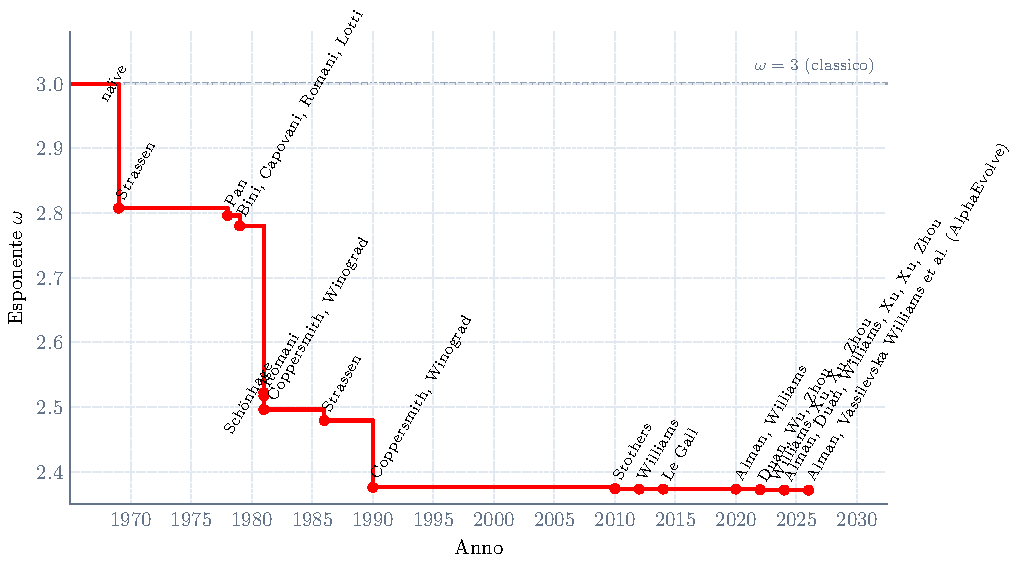
\includegraphics[width=0.9\textwidth, keepaspectratio]{Sources/Chapter3/figures/matrix_multiplication_timeline.pdf}
  \caption{Miglioramenti del limite superiore dell'esponente della moltiplicazione matriciale $\omega$ dal 1969 ad oggi. La linea tratteggiata rappresenta il limite superiore $\omega \le 3$.}
  \label{fig:matrix_mult_timeline}
\end{figure}

\begin{remark}
  Nella maggior parte della applicazioni, l'algoritmo di Strassen è quello ottimale, si
  veda la discussione in \cite{dalberto2023strassensmatrixmultiplicationalgorithm}. Di recente,
  il problema di stimare $ \omega $ e trovare il rango di tensori è diventato un problema
  d'interesse della branca della teoria della complessità algebrica e della geometria algebrica. Si
  veda ad esempio~\cite{landsberg2011tensors}.
\end{remark}


\section{Decomposizione low-rank di forme bilineari}

\todo{Spostare davanti alla CP per alleggerire (già scritta)}
Nel calcolo della complessità, le decomposizioni low-rank possono ridurre notevolmente le operazioni
aritmetiche sulle matrici. Se ad esempio $ M \in \R^{m\times n} $ è una matrice di rango uno, possiamo scrivere $ M =
u \topp v = uv^{\top} $ per certi $ u \in \R^m $ e $ v \in \R^n $; valutare $ Mx =
(uv^{\top})x = u(v^{\top}x) $ ha costo $ O(n) $, contro il costo $ O(mn) $ del prodotto classico
matrice vettore. In generale, se $ M $ ha rango $ R $, possiamo scriverla come somma di $ R $
matrici di rango uno\todo{aggiungere thm?} ed
ottenere un costo $ O(Rn) $ per $ Mx $. È possibile riadattare quest'idea per forme bilineari, come vedremo ora.

Calcolare la valutazione di una forma bilineare $ f $ come nell'Equazione~\ref{eq:b_k_bil} ha un costo $
  O(mnp) $, data dal numero di
  moltiplicazioni necessarie fra gli elementi di $ x $ e $ y $. Queste sono dette \emph{active
  multiplications} e corrispondono al numero di elementi non nulli di $ T $. Ci aspettiamo che
  la complessità di valutare $ f(x,y) $ sia correlata al costo delle active multiplications. Cerchiamo di minimizzarne il numero cercando fattorizzazioni CP di $ T $.


\begin{definition}[Bilinear algorithm]
  Sia $ \varphi : U \times V \to  W $ una mappa bilineare tra $ \K $-spazi vettoriali. Per ogni $ i
  \in \{1, \dots, r\} $, siano $ f_{i} \in U^*, g_{i} \in V^*, w_{i} \in W$ tali che
  \begin{equation*}
    \varphi(u,v) = \sum_{i=1}^r f_{i}(u)g_{i}(v)w_{i},
  \end{equation*}
  per ogni $ u \in U, v \in V$. Allora la $ r $-upla $ (f_1,g_1,w_1; \ldots ; f_r, g_r,w_r) $ viene
  detta \emph{bilinear computation (algorithm) di lunghezza $ r $ per $ \varphi $}, e la lunghezza
  di più breve algoritmo di calcolo per $ \varphi $ è chiamata \emph{bilinear complexity} o rango
  di $ \varphi $, che indichiamo ancora con $ \rk(\varphi) $.
\end{definition}


\begin{proposition}[Strassen]
  Siano $ U,V $ e $ W $ dei $ \K $-spazi vettoriali finiti, e $ \varphi : U\times V \to  W $ una
  mappa bilineare. Allora
  \begin{equation*}
    L(\varphi) = \text{Lunghezza della più breve bilinear computation per } \varphi.
  \end{equation*}
\end{proposition}
\begin{remark}
  Da questa proposizione segue direttamente che
  \begin{equation}
    \label{eq:LandRank_estimate}
    L(\varphi) \le \rk(\varphi) \le 2L(\varphi).
  \end{equation}
\end{remark}



La prossima definizione assicura che il rango di una forma bilineare è dato dal rango CP.
\begin{proposition}
  Fissata una forma bilineare $ \varphi $, e detto $ T $ il tensore che la rappresenta. Allora, dalla
  fattorizzazione CP di un tensore $ T $ si ottieme una bilinear computation, e in particolare $
  \rk(\varphi) = \rk(T) $.
\end{proposition}
\begin{proof}
Data una decomposizione $ T = \dsqr{U,V,W} $ di rango $ r $, dalla Definizione~\ref{def:CP}
abbiamo che $ T = \sum_{l=1}^r u_l \topp v_l \topp w_l $, o in componenti, $ T_{i,j,k} =
\sum_{l=1}^r u_{il}v_{jl}w_{kl} $. Inserendo questa relazione nell'Equazione~\ref{eq:b_k_bil} troviamo,

\begin{equation}
  \label{eq:b_active}
  \begin{aligned}
    \varphi_k(x,y) &= \left( \left( \sum_{l=1}^r u_l \topp v_l \topp w_l \right) \ttm[1] x^{\top} \ttm[2]
  y^{\top}  \right)_k  
             = \left( \sum_{l=1}^r \left( u_l \topp v_l \topp w_l  \right) \ttm[1] x^{\top} \ttm[2]
    y^{\top} \right)_k  \\ 
             &=
  \sum_{i=1}^m \sum_{j=1}^n \sum_{l=1}^r u_{il}v_{jl}w_{kl} x_i y_j = \sum_{l=1}^r \left(\sum_{i=1}^m 
    u_{il} x_i \right) \cdot \left( \sum_{j=1}^n v_{jl} y_j  \right)  w_{kl} \\
             &= \sum_{l=1}^r
   (u_l^{\top}x) \cdot (v_l^{\top}y)w_{kl},
  \end{aligned}
\end{equation}
per ogni $ k = 1, \ldots, p $.
Mettendo insieme le Equazioni \ref{eq:b_tuv} e \ref{eq:b_active} troviamo
\begin{equation}
  \label{eq:lowrank_bilinear}
  \varphi(x,y) = \sum_{l=1}^r (u_l^{\top}x)\cdot(v_l^{\top}y)w_l.
\end{equation}
Considerando i funzionali $ f_{l}(x) \defeq u_{l}^{\top}x $ e $ g_{l}(y) \defeq v_{l}^{\top}y $
indotti dal prodotto scalare standard si ha la tesi.

\end{proof}
Quindi valutare $ \varphi $ richiede esattamente $ r = \rk(T) $ active multiplications (e $
  O(r) $ addizioni), che sopra evidenziamo con $
(\cdot) $.
In particolare, il seguente risultato algebrico ci dice che la rappresentazione di una forma
bilineare come tensore o come bilinear computation sono identiche, ed è utile per riscrivere un
algoritmo tramite un tensore. 
\begin{proposition}[Si veda~\cite{burgisser2013algebraic}, Cap. 14]
  \label{prop:iso_bil_tensor}
  Siano $ U,V $ e $ W $ dei $ \K $-spazi vettoriali. Allora esiste un unico isomorfismo $ U^*
  \otimes V^* \otimes W \to \{\varphi : U \times V \to  W, \text{ bilineare}\} $ che manda $ f
  \otimes g \otimes w $ nella mappa bilineare $ (u,v) \mapsto f(u)g(u)w $.
\end{proposition}
\begin{definition}[Tensore strutturale]
  L'unico tensore $ T \in U^* \otimes V^* \otimes W$ associato alla mappa bilineare $ \varphi : U
  \times V \to W $ è detto \emph{tensore strutturale} di $ \varphi $.
\end{definition}


\section{Rappresentazione del prodotto tra matrici}

Consideriamo due matrici $ A \in \R^{M \times N} $ e $ B \in \R^{N \times P} $ e il loro prodotto $
C \in \R^{M \times P} $. Ponendo $ x =
\Vec(A) $ e $ y=\Vec(B) $, l'Equazione~\ref{eq:b_tuv} diventa 
\begin{equation}
  \label{eq:mulvec}
\Vec(C^\top) =\varphi(x,y) = T \ttm[1] \Vec(A)^{\top} \ttm[2] \Vec(B)^{\top}
,\end{equation}

dove abbiamo fissato l'ordinamento naturale sulle entrate di $ \Vec(A) $ e $ \Vec(B) $, e quello
inverso su $
\Vec(C^\top)$. Da ciò troviamo un tensore $ T \in \R^{MN\times NP\times MP} $ che rappresenta
la moltiplicazione tra $ \algob{M,N,P} $.
Data una decomposizione CP di rango $ r $ del tensore $ T  = \dsqr{U,V,W}$,
grazie all'Equazione~\ref{eq:lowrank_bilinear}, l'espressione sopra si traduce in
\begin{equation}
  \label{eq:mulvec:CP}
  \Vec(C^\top) =  \sum_{l=1}^r (u_l^\top \Vec(A)) \cdot
  (v_l^\top\Vec(B))w_l = \sum_{l=1}^r (s_l \cdot
  t_l)w_l = \sum_{l=1}^r m_lw_l,
\end{equation}
Dove abbiamo posto $ s_l \defeq  s_{l}(A) \defeq  u_l^\top \Vec(A)$, $ t_l \defeq t_{l}(B) \defeq v_l^\top\Vec(B)$ e $ m_l \defeq
s_lt_l $. Nella pratica, nei passaggi successivi dell'algoritmo calcoliamo in maniera ricorsiva il
prodotto tra $ s_l $ e $ t_l $.
Questa formula definisce un algoritmo di moltiplicazione veloce $ \algob{M,N,P} $.

\begin{figure}[htbp]
  \centering
  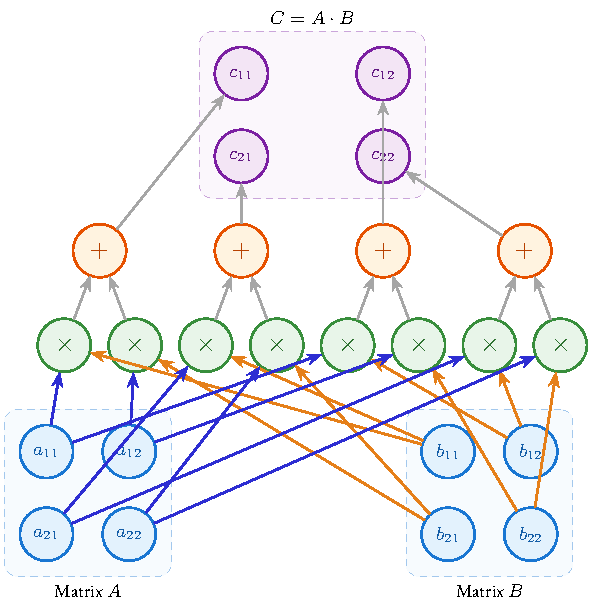
\includegraphics{Sources/Chapter3/figures/circuit.pdf}
  \caption{Circuito aritmetico per la moltiplicazione di matrici $2 \times 2$.}
  \label{fig:arithmetic_circuit_222}
\end{figure}


\section{Alcune stime sull'esponente}
\label{sec:exp_estimates}
Dal ragionamento sopra, $ \rk(\algob{n}) $ è dato dal numero di active multiplication nella molitiplicazione
di due matrici, e quindi ne misura la complessità algoritmica. Possiamo quindi riscrivere $ \omega $ come
\begin{equation}
  \label{eq:omega_as_rank}
  \omega = \lowlim_{n \to +\infty} \log_n \left( \rk(\algob{n}) \right).
\end{equation}
\todo{FIX errore nella formula}
Ad esempio, l'algoritmo di Strassen~\cite{strassen69} mostra che $ \rk(\algob{2}) \le 7$, e
come dimostrato da Winograd~\cite{winograd1971}, $ \rk(\algob{2}) = 7$, ovvero non è possibile moltiplicare due
matrici $ 2\times 2 $ con meno di sette moltiplicazioni.
Nei casi diversi da $ \algob{2} $ il problema si complica, e attualmente abbiamo alcune stime più lasche: già
per matrici $ 3\times 3 $, sappiamo solo che $ 19 \le \rk(\algob{3}) \le 23 $~\cite{BLASER200343,
bams/1183537626}, mentre la migliore stima astintotica dal basso per il caso di matrici $ n\times n $ è $ \frac{5}{2}n^2 - 3n \le
\rk(\algob{n}) $~\cite{blaser2001}. Si veda il capitolo 11 di~\cite{landsberg2011tensors} per
ulteriori dettagli e stime.


\subsection*{Trattare il caso generale}

Date due matrici $ n^i \times n^i $, possiamo vedere la loro moltiplicazione come la moltiplicazione
di matrici $ n\times n $ sull'algebra delle matrici $ n^{i-1}\times
n^{i-1} $, suddividendole in blocchi. Questo dice anche che, se $
\rk(\algob{n}) \le r $, allora $ \rk(\algob{n^i}) \le
  r^i$; infatti, combinando le prossime Proposizioni~\ref{prop:bil_map_product}
e~\ref{prop:rk_bil_map_product}, e usando che il rango è invariante per isomorfismo, troviamo
\begin{equation*}
  \rk(\algob{n^i}) = \rk(\algob{n}^{\otimes i}) \le \rk(\algob{n})^i \le r^i.
\end{equation*}
Quindi, possiamo applicare ricorsivamente l'algoritmo di moltiplicazione veloce, che è disegnato per
matrici $ n\times n $, per ottenere la moltiplicazione di matrici $ n^i \times n^i $ impiegando solo $ r^i $ moltiplicazioni.

Se invece $ n > n_0 $ sono due interi positivi, dato un algoritmo con un caso base fissato $
\algob{n_0} $, è possibile ottenerne uno per
$ \algob{n} $, con $ n >  n_0 $, allargando la matrice aggiungendo zeri
fino alla dimensione
$ n_0^{\left\lceil \log_{n_0} n \right\rceil } $. La complessità dipenderà comunque da $ n_0 $ e
da $ r $, in quanto
\begin{equation*}
  \begin{aligned}
    \rk(\algob{n}) &\le \rk(\algob{n_0^{\left\lceil \log_{n_0} n \right\rceil }}) && \text{dalla
    \ref{prop:rk_monotony},} \\
                  &\le \rk(\algob{n_0})^{\left\lceil \log_{n_0} n \right\rceil } && \text{dalle
    \ref{prop:bil_map_product} e \ref{prop:rk_bil_map_product},}\\
                  &\le r^{\left\lceil \log_{n_0} n \right\rceil } && \text{per ipotesi $
  \rk(\algob{n}\le r $,} \\
                  &\le r \cdot n^{\log_{n_0} r} && \text{usando che $ \left\lceil x \right\rceil \le
                  x+1$}.
  \end{aligned}
\end{equation*}
Riassumendo, $ \rk(\algob{n,n,n}) \le r \cdot n^{\log_{n_0} r} $. Dunque ignorando la costante e
dall'Equazione~\ref{eq:omega_as_rank}, $ \omega \le \log_{n_0} r $. Ad esempio, per
l'algoritmo di Strassen poniamo $ r = 7,n_0 = 2 $, da cui $ \omega \le \log_{2} 7 < 2.81 $. Abbiamo
dimostrato la seguente:
\begin{proposition}
  Se $ \rk(\algob{n}) \le r$ per degli interi positivi $ n,r $, allora $ n^\omega \le r $.
\end{proposition}

Nei passaggi sopra abbiamo anche osservato che se $ n \le n' $ e dato un algoritmo per $ n' $, possiamo ottenerne uno per $ n $
allargando la matrice. Possiamo racchiudere questa proprietà nel seguente risultato:
\begin{proposition}[Monotonia del rango di un algoritmo]
  \label{prop:rk_monotony}
Il rango di un algoritmo è monotono crescente rispetto alla dimensione, ovvero dati due interi positivi $ n \le n' $, allora $
\rk(\algob{n}) \le \rk(\algob{n'}) $.
\end{proposition}



Riportiamo le proposizioni utilizzate per dimostrare la proposizione sopra, dimostrate
in~\cite{burgisser2013algebraic}, Cap. 14,15.
\begin{proposition}
  \label{prop:bil_map_product}
  Siano $ e,e', h,h',l,l' $ degli interi positivi. Allora abbiamo
  \begin{equation*}
    \algob{e,h,l} \otimes \algob{e', h', l'}\simeq \algob{ee', hh', ll'},
  \end{equation*}
  cioè le due forme bilineari sono isomorfe.
\end{proposition}
\begin{proposition}
  \label{prop:rk_bil_map_product}
  Siamo $ \varphi_1,\varphi_2 $ due mappe bilineari. Allora $ \rk(\varphi_1 \otimes \varphi_{2}) \le
  \rk(\varphi_1)\rk(\varphi_2)$.
\end{proposition}

\section{Il rango come misura della complessità}

% La condizione trovata nell'Equazione~\ref{eq:omega_as_rank} è anche necessaria \todo{check}. 
La prossima proposizione mostra che il rango di un tensore è una misura ottimale della complessità.
Inoltre risponde all'esistenza del problema inverso: dato un intero positivo $ r $, è possibile
trovare un algoritmo con $ r $ moltiplicazioni? La risposta precisa è data dal seguente risultato.
\begin{theorem}[Strassen~\cite{strassen69}, vedi anche \cite{burgisser2013algebraic} §15.1]
  \label{thm:strassen}
  \begin{equation*}
    \omega = \inf \{\tau \in \R \mid \rk(\algob{n}) = O(n^\tau)\}.
  \end{equation*}
  Ovvero, è possibile moltiplicare due matrici $ n\times n $ usando $ O(n^{\omega + \varepsilon}) $
  operazioni aritmetiche se e solo se il rango tensoriale di $ \algob{n} $ è $
  O(n^{\omega+\varepsilon}) $.
\end{theorem}

Introduciamo alcuni strumenti utili a dimostrare questo risultato.
\begin{definition}[Mappa bilineare concise]
  Sia $ \varphi : U\times V \to  W$ una mappa bilineare. Diremo che $ \varphi $ è \emph{concise} se
  valgono tutte e tre le condizioni sotto:
  \todo{change to roman and to $ i $-concise per matchare quella dei tensori}
  \begin{enumerate}
    \item $\lKer(\varphi) = \{u \in U \mid \varphi(u,\cdot ) = 0\}  = \{0\} $,
    \item $\rKer(\varphi) = \{v \in V \mid \varphi(\cdot,v ) = 0\}  = \{0\} $,
    \item $\Im(\varphi) = \{\varphi(u,v) \mid u\in U, v\in V\} = W$.
  \end{enumerate}
\end{definition}
\begin{remark}
  \todo{osservare che combacia con la def data per i tensori}
\end{remark}
\begin{example}
  La mappa bilineare $ \algob{n} $ è concise.
\end{example}

\begin{lemma}
  \label{lemma:rec_relation_ab}
  Sia $ x = \left( x_0, x_1, x_2,\ldots \right) $ una successione di numeri reali che soddisfa la
  ricorsione $ x_s = ax_{s-1} + cb^s $, per certi numeri reali $ a,b,c $. Allora per ogni $ s \ge 0
  $, vale
  \begin{equation*}
    x_s = \begin{cases}
      a^s x_0 + (a^s - b^s) \frac{bc}{a-b} & \text{se } a\neq b, \\
      (cs + x_0)a^s & \text{se } a = b.
    \end{cases}
  \end{equation*}
\end{lemma}
\begin{proof}
  Mostriamo la formula per induzione su $ s $. Per $ s=0 $ la formula è verificata.
  \begin{equation*}
    \begin{aligned}
    x_1 &= ax_0 + bc, \\
    x_2 &= a(ax_0 + bc) + b^2 c \\
        &= a^2 x_0 + (a + b)bc \\
        &= \begin{cases}
          a^2x_0 + (a^2 - b^2)\frac{bc}{a-b} & \text{se } a\neq b, \\
          (2c + x_0)a^2 & \text{se } a=b.
        \end{cases}
    \end{aligned}
  \end{equation*}
  Assumiamo la proprietà vera per $ n-1 $ e mostriamola per $ n $.

  Se $ a \neq b $, 
  \begin{equation*}
    \begin{aligned}
      x_s &= a\left(a^{s-1}x_0 + \left(a^{s-1} - b^{s-1}\right) \frac{bc}{a-b}\right) + b^sc \\
          &= a^s x_0 + \left( (a^{s-1} - b^{s-1})a + b^{s-1}(a-b) \right)\frac{bc}{a-b} \\
          &= a^s x_0 + \left(a^{s}-b^{s} \right)\frac{bc}{a-b}
    \end{aligned}
  \end{equation*}

  Similmente, se $ a = b $
  \begin{equation*}
    \begin{aligned}
      x_s &= \left( c(s-1) + x_0 + c \right)a^s \\
          &=  (cs + x_0)a^s.
    \end{aligned}
  \end{equation*}
\end{proof}

\begin{proof}[Dimostrazione del Teorema di Strassen]
  Dimostriamo che 
  \begin{equation*}
    \omega = \inf \{\tau \in \R \mid \rk(\algob{n}) = O(n^\tau)\}.
  \end{equation*}
  Sia $ \theta $ il lato destro dell'equazione sopra, e per semplicità scriviamo $ M(n) \defeq
  M_{\K}(n)$ e $ \omega \defeq \omega_{\K}$. Dall'Equazione~\ref{eq:LandRank_estimate} abbiamo
  \begin{equation*}
    \frac{1}{2}R(\algob{n}) \le L(\algob{n}) \le M(n),
  \end{equation*}
  e dalla Definizione~\ref{def:exponent_matmul} segue $ \theta \le \omega $.

  Mostriamo che $ \omega \le \theta $. Per definizione di $ \theta $, per ogni $ \varepsilon >0 $
  esiste un $ n>1 $ tale che
  \begin{equation}
    \label{eq:r_estimate}
    r \defeq \rk(\algob{n}) \le n^{\theta + \varepsilon}.
  \end{equation}
  
  Dall'Equazione~\ref{eq:mulvec:CP}\todo{matrix product, ma TODO verifica, e controlla se è così davvero( io ho i vec)} esistono dei funzionali $ f_{\rho},g_{\rho} \in
  (\K^{n\times n})^*$  e delle matrici $ w_{\rho} \in \K^{n\times n} $ per $ \rho \in \{1, \ldots,
  r\}  $ tali che, per ogni $ A,B \in \K^{n\times n} $
  \begin{equation*}
    AB = \sum_{\rho = 1}^r f_{\rho}(A)g_{\rho}(B) w_{\rho}.
  \end{equation*}
  Vedendo $ \mathcal{A} = \K^{n^i\times n^i} $ come l'algebra delle matrici $ n^i \times n^i $, notiamo che i funzionali $ f_{\rho}, g_{\rho} : \K^{n\times n} \to \K $ si estendono a funzionali
  $ f_{\rho}, g_{\rho} : \mathcal{A}^{n\times n} \to \mathcal{A} $, sostituendo le entrate scalari
  con delle matrici. In particolare vale, per ogni $ A,B \in \mathcal{A}^{n\times n} $
  \begin{equation}
    \label{eq:blk_matmul_algo}
    AB = \sum_{\rho = 1}^r f_{\rho}(A)g_{\rho}(B) w_{\rho}.
  \end{equation}
L'Equazione sopra rappresenta l'algoritmo di moltiplicazione a blocchi tra $ A
  $ e $ B $: infatti abbiamo $ \mathcal{A}^{n\times n} = (\K^{n^i\times n^i})^{n \times n} \simeq \K^{n^{i+1}
  \times n^{i+1}} $, dove l'isomorfismo è dato dalla decomposizione in blocchi. Da questo fatto,
  unito all'Equazione~\ref{eq:blk_matmul_algo}, si
  ottiene che
  \begin{equation}
    \label{eq:Mn_recursionleq}
    M(n^{i+1}) \le r M(n^i) + cn^{2i},
  \end{equation}
  dove $ c \defeq c(n,r) $ è una costante che dipende sia da $ n $ che da $ r $. Questo perché nella
  formula il prodotto $ AB $, sviluppato come prodotto tra blocchi $ n^i \times n^i $ (formalmente, visto come prododotto a coefficienti in $ \mathcal{A} $), coinvolge $ r $ prodotti e
  un numero costante di addizioni.
  Siccome $ \algob{n} $ è concise, abbiamo che $ r \ge n^2 $. Fissando $ n $ (e quindi $ r $),
  risolviamo la ricorsione dell'Equazione~\ref{eq:Mn_recursionleq} in funzione di $ i $ usando il
  Lemma~\ref{lemma:rec_relation_ab} con $ a = r $ e $ b = n^2 $, analizzando due casi.

  Se $ r > n^2 $, abbiamo che
  \begin{equation*}
    \begin{aligned}
      M(n^i) &= r^i M(1) + (r^i - n^{2i})\frac{n^2c}{r-n^2} \\
             &= (M(1) + n^2c)r^i - n^{2i}\frac{n^2c}{r-n^2},
    \end{aligned}
  \end{equation*}
  da cui, 
  \begin{equation*}
    M(n^i) \le \alpha r^i + \beta n^{2i},
  \end{equation*}
  dove abbiamo posto $ \alpha \defeq M(1) + n^2c $ e $ \beta \defeq - \frac{n^2c}{r-n^2}$. 

  Se $ r = n^2 $, dal Lemma~\ref{eq:Mn_recursionleq} abbiamo
  \begin{equation*}
    M(n^i) \le (cs + M(1))r^i,
  \end{equation*}

  In entrambi i casi troviamo,
  \begin{equation}
    \label{eq:Mn_as_O_ri}
    M(n^i) = O(r^i).
  \end{equation}
  Dalla proposizione~\ref{prop:rk_monotony} segue che $M$ è una successione monotona, da cui per ogni $ h = n^i \in \N \setminus \{0\}  $, 
  \begin{equation*}
    M(h) = O(r^{\log_{n}h}) = O(h^{\log_{n}r}) = O(h^{\theta + \varepsilon}),
  \end{equation*}
  dove la prima uguaglianza segue sostituendo, $ i = \log_n h$
  nell'Equazione~\ref{eq:Mn_recursionleq}, la seconda da una proprietà del logaritmo, e la terza
  applicando la stima dell'Equazione~\ref{eq:r_estimate}.
  Quindi $ \omega_{\K} \le \theta $, che completa la dimostrazione.
\end{proof}

\section{Algoritmi di moltiplicazione veloce}

\begin{remark}
  \label{rem:rectangular}
  Di seguito ci limiteremo a studiare prodotti fra matrici quadrate; per il caso rettangolare, si
  possono estendere i ragionamenti sopra considerando una rappresentazione di rango $ r $ del
  tensore $ \algob{m,n,p} $ e scrivendo, attraverso una serie di permutazioni cicliche, la fattorizzazione di $ \algob{mnp} $ di rango $ r^3 $, che produce un algoritmo di complessità $ O(n^{\log_{abc}r^3}) =
  O(n^{3\log_{abc}r})$. Questo si può vedere tramite la scrittura della moltiplicazione tra matrici
  come forma trilineare dell'Osservazione~\ref{rmk:triliear_matmul} ci assicura che il tensore è
  invariante per trasformazioni cicliche, in quanto
  \begin{equation}
    \mathop{trace}(ABC) = \mathop{trace}(CAB) = \mathop{trace}(BAC).
  \end{equation}
\end{remark}


\subsection*{Il caso naive}
\todo{Dire se la derivazione del tensore è chiara, ho provato a giustificarla meglio che potessi}

Trattiamo il caso di matrici quadrate con taglie potenze di due (possiamo farlo a meno di passare a
una sottomatrice di taglia pari). In questo caso possiamo
partizionare le matrici in delle sottomatrici a blocchi $ 2\times 2 $ \footnote{possiamo pensare alle entrate
sia come scalari, che come matrici.}:
\begin{equation*}
  \begin{bmatrix}
    c_{11} & c_{12} \\
    c_{21} & c_{22}
  \end{bmatrix} =
  \begin{bmatrix}
    a_{11} & a_{12} \\
    a_{21} & a_{22}
  \end{bmatrix} \cdot 
  \begin{bmatrix}
    b_{11} & b_{12} \\
    b_{21} & b_{22}
  \end{bmatrix} =
  \begin{bmatrix}
    a_{11}b_{11} + a_{12}b_{21} & a_{11}b_{12} + a_{12}b_{22} \\
    a_{21}b_{11} + a_{22}b_{21} & a_{21}b_{12} + a_{22}b_{22}
  \end{bmatrix}.
\end{equation*}
L'algoritmo naive procede combinando un insieme di otto moltiplicazioni matriciali con quattro
addizioni:

\begin{equation}
\label{eq:mult_222_m_i}  
\begin{aligned}
m_1 &= a_{11} \cdot b_{11} = s_1 t_1&\quad m_2 &= a_{12} \cdot b_{21} = s_2t_2 &\quad m_3 &= a_{11}
\cdot b_{12} = s_3t_3 \\
m_4 &= a_{12} \cdot b_{22} = s_4t_4 &\quad m_5 &= a_{21} \cdot b_{11} = s_5t_5 &\quad m_6 &= a_{22}
\cdot b_{21} = s_6t_6 \\
m_7 &= a_{21} \cdot b_{12} = s_7t_7 &\quad m_8 &= a_{22} \cdot b_{22} = s_8t_8 & &
\end{aligned}
\end{equation}

\[
\begin{aligned}
 c_{11} &= m_1 + m_2 = a_{11}b_{11} + a_{12}b_{21}, &\qquad  c_{12} &= m_3 + m_4 = a_{11}b_{12} +
a_{12}b_{22}, \\
 c_{21} &= m_5 + m_6 = a_{21}b_{11} + a_{22}b_{21}, &\qquad  c_{22} &= m_7 + m_8 = a_{21}b_{12} +
a_{22}b_{22}.
\end{aligned}
\]

\begin{figure}[htbp]
  \centering
  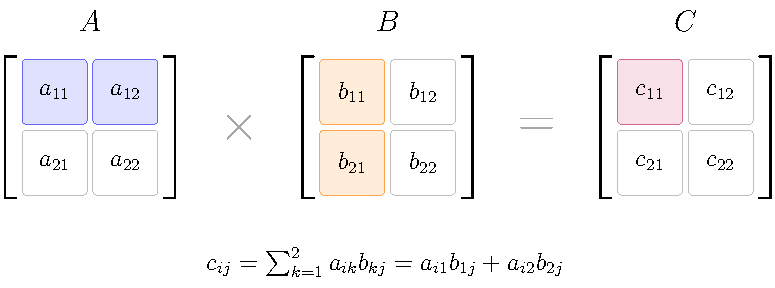
\includegraphics{Sources/Chapter3/figures/matrix_multiplication_linear.pdf}
  \caption{Rappresentazione della moltiplicazione di due matrici $2 \times 2$.}
  \label{fig:matrix_multiplication_linear}
\end{figure}

Proviamo a scriverlo in forma tensoriale. La sua bilinear computation è
\begin{equation*}
  C = \sum_{i=1}^8 m_{i}w_{i}
\end{equation*}
Usando l'Osservazione~\ref{rmk:triliear_matmul} possiamo scrivere $ \algob{2} $ come mappa
trilineare come
\begin{equation*}
  \begin{aligned}
    \mathop{trace}(ABC) &= 
    \mathop{trace}\left(
    \begin{bmatrix} 
    s_1t_1 + s_2t_2 & s_3t_3 + s_4t_4 \\
    s_5t_5 + s_6t_6 & s_7t_7 + s_8t_8
    \end{bmatrix} 
    \begin{bmatrix} c_{11} & c_{12} \\ c_{21} & c_{22} \end{bmatrix} 
    \right) \\
                           &= (s_1t_1 + s_2t_2)c_{11} + (s_3t_3 + s_4t_4)c_{21}+ (s_5t_5 +
                           s_6t_6)c_{12} + (s_7t_7 + s_8t_8)c_{22}.
  \end{aligned}
\end{equation*}
Tramite l'isomorfismo della Proposizione~\ref{prop:iso_bil_tensor}, possiamo mappare ogni termine $
s_{r}t_{r}w_{r}$ dell'equazione sopra in $ s_{r} \otimes t_{r} \otimes c_{r}$ e scrivere il tensore struttrale di $
\algob{2} $ in formato CP:
e visualizzarlo nella Figura~\ref{fig:tensor_222_cp}:
\begin{equation}
  \label{eq:tensor_222}
  \begin{aligned}
    \algob{2} &= a_{11} \topp b_{11}\topp c_{11} + a_{12}\topp b_{21} \topp c_{11} \\
                 &+ a_{21}\topp b_{11} \topp c_{21} + a_{22} \topp b_{21} \topp c_{21} \\ 
                 &+ a_{11} \topp b_{12} \topp c_{12} + a_{12} \topp b_{22} \topp c_{12} \\
    &+ a_{21} \topp b_{12} \topp c_{22} + a_{22}\topp b_{22}\topp c_{22}.
  \end{aligned}
\end{equation}


\begin{figure}[htbp]
  \centering
  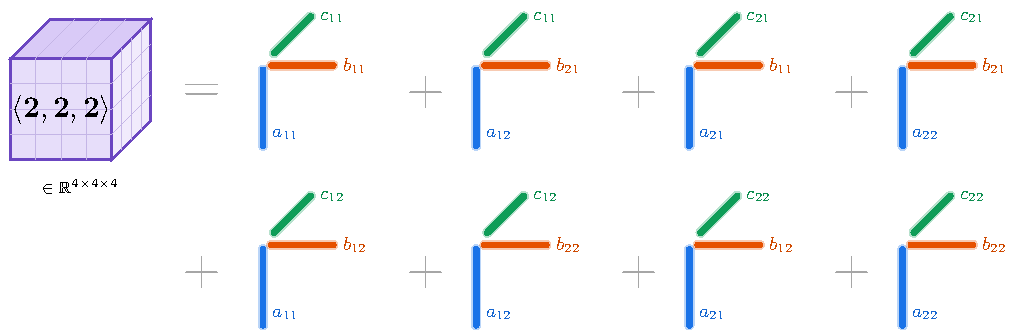
\includegraphics[width=\textwidth]{Sources/Chapter3/figures/tensor_222_cp.pdf}
  \caption{Decomposizione CP del tensore di moltiplicazione di matrici $ \algob{2} $ come somma di 8 tensori di rango uno.}
  \label{fig:tensor_222_cp}
\end{figure}



Per secoli questo algoritmo è stato ritenuto il più veloce per moltiplicare le matrici. Nel ??
Strassen \footnote{in una comunicazione riportata da Landsberg in~\cite{landsberg2011tensors}.}
tentò di mostrare che non esistesse un algoritmo più veloce, fallendo in maniera spettacolare \footnote{in realtà
la tesi è vera nel campo $ \Z/2\Z $.} e dando vita a una nuova teoria.

\subsection*{L'algoritmo di Strassen}

L'algoritmo di Strassen è probabilmente l'algoritmo di moltiplicazione veloce più noto e segue la
stessa struttura a blocchi $ \algob{2} $.

\begin{align*}
s_1 &= a_{11} + a_{22} & s_2 &= a_{21} + a_{22} & s_3 &= a_{11} \\
s_4 &= a_{22} & s_5 &= a_{11} + a_{12} & s_6 &= a_{21} - a_{11} \\
s_7 &= a_{12} - a_{22} \\
t_1 &= b_{11} + b_{22} & t_2 &= b_{11} & t_3 &= b_{12} - b_{22} \\
t_4 &= b_{21} - b_{11} & t_5 &= b_{22} &t_6 &= b_{11} + b_{12} \\
t_7 &= b_{21} + b_{22}
\end{align*}
\begin{align*}
m_r &= s_rt_r, \quad 1 \le r \le 7 \\
c_{11} &= m_1 + m_4 - m_5 + m_7 & c_{12} &= m_3 + m_5 \\
c_{21} &= m_2 + m_4 & c_{22} &= m_1 - m_2 + m_3 + m_6
\end{align*}

\todo{Aggiungere tensore}
\todo{aggiungere costo}

\section{Algoritmi APA}
\label{sec:APA}

Dopo il tentativo di Strassen di dimostrare che l'algoritmo di moltiplicazione standard fosse
ottimale, Bini et. Al~\cite{bini1980relations} considerano il seguente algoritmo di moltiplicazione ridotto ottenuto
ponendo a zero l'entrata $ a_{22} $ di $ \algob{2} $:
\begin{equation*}
  \begin{bmatrix}
    a_{11} & a_{12} \\
    a_{21} & 0
  \end{bmatrix} \cdot 
  \begin{bmatrix}
    b_{11} & b_{12} \\
    b_{21} & b_{22}
  \end{bmatrix} =
  \begin{bmatrix}
    a_{11}b_{11} + a_{12}b_{21} & a_{11}b_{12} + a_{12}b_{22} \\
    a_{21}b_{11}  & a_{21}b_{12} 
  \end{bmatrix}.
\end{equation*}
Facendo alcuni raccoglimenti e sostituendo $ a_{22} =0$, il tensore dell'Equazione~\ref{eq:tensor_222} si riscrive come
\begin{equation*}
  \begin{aligned}
    \algob{2}^{\text{red}}
    &\defeq a_{11} \topp (b_{11} \topp c_{11} + b_{12} \topp c_{12})
                              + a_{12} \topp (b_{21} \topp c_{11} + b_{22} \topp c_{12})\\ 
                              &+ a_{21} \topp (b_{11} \topp c_{21} + b_{12}
  \topp c_{22}).
  \end{aligned}
\end{equation*}

Che è somma di sei tensori elementari distinti, quindi $ \rk{\algob{2}^{\text{red}}} \le 6 $.
Bini et. al. provarono a cercare un'espressione di rango cinque per $ \algob{2}^{\text{red}} $
numericamente, calcolando
\begin{equation*}
  \min_{\substack{T \in \R^{n\times n\times n} \\ \rk(T) = 5}}{\| \algob{2}^{\text{red}} - T\| }
\end{equation*}
 norma di $ \algob{2}^{\text{red}} $. Il loro computer continuava a produrre tensori $ T $ di rango cinque
con la norma della differenza che diventava sempre più piccola, ma con coefficienti sempre più
grandi. Questo è andato avanti per un po' di tempo, fino a che realizzarono che il codice era
giusto, ma quello che sembrava un problema era in realtà una manifestazione di un fenomeno chiamato \emph{border rank}.
L'espressione del tensore che stavano cercando era il seguente tensore di rango $ 5 $:
\begin{equation*}
  \begin{aligned}
    \algob{n}_t^{\text{red}} = \frac{1}{t} \left[ (I) + (II) -(III) - (IV) + (V)
    \right],
  \end{aligned}
\end{equation*}
dove 
\begin{equation*}
  \begin{aligned}
    (I) &= (x_2^1 + tx_1^1) \otimes (y_2^1 + ty_2^2 \otimes z_2^1) \\
        &= x_{2}^1 \otimes y_2^1 \otimes z_2^1 + t[x_2^1 \otimes y_2^2 \otimes z_2^1 + x_1^1 \otimes
        y_2^1 \otimes z_2^1] + O(t^2) \\
    (II) &= (x_1^2 + tx_1^1) \otimes y_1^1 \otimes (z_1^1 + tz_1^2) \\
         &= x_1^2 \otimes y_1^1 \otimes z_1^1 +t[x_1^2 \otimes y_1^1 \otimes z_1^2 + x_1^1 \otimes
         y_1^1 \otimes z_1^1] + O(t^2) \\
    (III) &= x_1^2 \otimes y_1^1 \otimes z_1^1 + t[x_1^2 \otimes y_1^1 \otimes z_1^2 + x_1^1 \otimes
    y_1^1 \otimes z_1^1] + O(t^2) \\
    (IV) &= x_1^2 \otimes ((y_1^1 + y_2^1) + ty_1^2) \otimes z_1^1 \\
         &= x_1^2 \otimes y_1^1 \otimes z_1^1 + x_1^2 \otimes y_2^1 \otimes z_1^1 + t[x_1^2 \otimes
         y_1^2 \otimes z_1^1] \\
    (V) &= (x_2^1 + x_1^2) \otimes (y_2^1 + ty_1^2) \otimes (z_1^1 + tz_2^2) \\
        &=x_2^1\otimes y_2^1 \otimes z_1^1 + x_1^2 \otimes y_2^1 \otimes z_1^1 \\
        &+ t[x_2^1 \otimes
        (y_2^1 + z_2^2 + y_1^2 \otimes z_1^1) + x_1^2 \otimes (y_2^1 \otimes z_2^2 + y_1^2 \otimes
        z_1^1)] + O(t^2)
  \end{aligned}
\end{equation*}
In ogni passaggio abbiamo applicato più volte la proprietà distributiva del prodotto tensoriale.
Osserviamo che i termini di grado costante in $ t $ si cancellano:
\begin{equation*}
  \begin{aligned}
    x_2^1 &\otimes (y_2^1 \otimes z_2^1 - y_2^1 \otimes z_1^1 - y_2^1 \otimes z_2^1 + y_2^1 \otimes
    z_1^1) \\
    + x_1^2 &\otimes (y_1^1 \otimes z_1^1 - y_1^1 \otimes z_1^1 + y_2^1 \otimes z_1^1 - y_2^1 \otimes z_1^1)
    = 0
  \end{aligned}
\end{equation*}
Sommando e raggruppando i termini di grado uno in $ t $ troviamo
\begin{equation*}
  \begin{aligned}
   \algob{n}^\text{red} = x_1^1 &\otimes (y_1^1 \otimes z_1^1 + y_2^1 \otimes z_2^1) +\\
    x_2^1 &\otimes (y_1^2 \otimes z_1^1 + y_2^2 \otimes z_2^1) + \\
    x_1^2 &\otimes (y_1^1 \otimes z_1^2 + y_2^1 \otimes z_2^2),
  \end{aligned}
\end{equation*}
ovvero il tensore di partenza. Da cui,
\begin{equation*}
  \algob{n}_t^{\text{red}} - \algob{n}^{\text{red}} = O(t^2) \to 0
\end{equation*}
Abbiamo dimostrato che un tensore di rango $ 5 $ converge a uno di rango $ 6 $.

\subsection*{Il problema del border rank}
\label{sec:border_rank}

\todo{Introduci e motiva il problema partendo dagli algoritmi APA (vedi Landsbeg)}

\begin{example}
  \label{ex:border_rank}
  Consideriamo dei vettori $ a_1,a_2 \in \R^m$, $b_1,b_2 \in \R^n$ e $c_1,c_2\in \R^p $ vettori
  linearmente indipendenti. Definiamo il tensore 
  \begin{equation}
    T = a_1 \topp  b_1 \topp c_2 + a_1 \topp b_2 \topp c_1 + a_2 \topp b_1 \topp c_1,
  \end{equation}
  e notiamo che $ \rk(T) = 3 $ dato che non può
  essere scomposto come somma di tensori più semplici.
  Consideriamo la successioni di tensori 
  \begin{equation}
  \label{eq:rank_counterex}
  T_\varepsilon = \frac{1}{\varepsilon}\left( a_1 +
  \varepsilon a_2 \right) \topp (b_1 + \varepsilon b_2) \topp (c_1 + \varepsilon c_2) -
  \frac{1}{\varepsilon} a_1 \topp b_1 \topp c_1, \text{ con } \varepsilon \in \R,
  \end{equation}
  che essendo combinazione lineare di due tensori di rango uno, ha rango 2.
  Vediamo che $ \lim_{\varepsilon \to 0} T_\varepsilon = T $, da cui segue che l'insieme dei tensori di rango 3 non è chiuso.
  Espandendo i termini dell'Equazione \ref{eq:rank_counterex} tramite la proprietà distributiva del prodotto esterno,
  \begin{equation}
    \begin{aligned}
      \Tn{y}_\varepsilon &=  \frac{1}{\varepsilon} a_1 \topp b_1 \topp c_2 + a_1 \topp b_1 \topp c_2 + a_1 \topp b_2 \topp c_1
      +a_2 \topp b_1 \topp c_1  \\ &+ \varepsilon \left(a_2 \topp b_2 \topp c_1 + a_1 \topp b_1 \topp c_2 +
      a_1 \topp b_2 \topp c_2 + a_2 \topp b_2 \topp c_2 \right) - \frac{1}{\varepsilon} a_1 \topp
      b_1 \topp c_1 \\
                         &= T + \varepsilon\left(a_2 \topp b_2 \topp c_1 + a_1 \topp b_1 \topp c_2 +
      a_1 \topp b_2 \topp c_2 + a_2 \topp b_2 \topp c_2 \right)
    \end{aligned}
  \end{equation}
  Quindi $ T_\varepsilon - T \to 0 $.
\end{example}

Questo motiva la seguente definizione:


\begin{definition}[Border rank]
  Un tensore $ T $ ha \emph{border rank} $ r $ se è limite di una successione di tensori di
  rango $ r $, ma non è limite di una successione di tesori di rango $ s $, per ogni $ s < r $. Lo
  denoteremo con il simbolo $ \brk(T) $.
\end{definition}
\begin{remark}
  $ \rk(T) \ge \brk(T) $.
\end{remark}
\begin{remark}
  In coordinate, se $ T \in \Rmsiz $, il suo border rank è la quantità
  \[
  \brk(T) = \min \left\{ r \in \N \mid \exists T' \in \Rmsiz! \text{ tale che }
  \rk(T')=r, \, \|T - T'\|  < \varepsilon \right\}
  .\] 
\end{remark}
\todo{Disegno interpretazione geometrica (landsberg pg 38)}

Il border rank si rivela utilissimo nello studio dell'esponente $ \omega $, cioè possiamo sostituire
il rango con il border rank nel Teorema~\ref{thm:strassen}:
\begin{theorem}[Bini~\cite{bini1980relations}, vedi \S3.2]
  \begin{equation*}
    \omega = \inf \{\tau \in \R \mid \brk(\algob{n}) = O(n^\tau)\} .
  \end{equation*}
\end{theorem}
Anche se potremmo avere $ \brk(\algob{n}) < \rk(\algob{n}) $, non sono abbastanza diversi da
avere un impatto sull'esponente\todo{why?}.

Riportiamo alcune stime sul border rank riportate in~\cite{landsberg2015geometry}, \S1. Per $ n = 2 $,
Winograd dimostra\todo{ref} che $ \brk(\algob{2}) = \rk(\algob{2}) = 7 $. Ci aspetteremmo che per $
n > 2 $, $ \brk(\algob{n}) < \rk(\algob{n}) $. Per $ n=3 $, sappiamo solo che $ 15 \le
\brk(\algob{3}) \le 20 $ e $ 19 \le \rk(\algob{3}) \le 23 $. In generale, sappiamo che $
\rk(\algob{n}) \ge  3n^2 - o(n) $ e $ \brk(\algob{n}) \ge 2n^2 - \left\lceil \log_{2}(n)
\right\rceil -1 $.

\section{Errore algoritmico}

\todo{discussione della stabilità dal paper dato dal prof}
